%%%%%%%%%%%%
%
% $Autor: Sudeshna,Srikanth Nanda, Adhiraj $
% $Datum: 2025-01-14 08:03:15Z $
% $Pfad: TemplateSensor $
% $Version: 4250 $
% !TeX spellcheck = en_GB/de_DE
% !TeX encoding = utf8
% !TeX root = filename 
% !TeX TXS-program:bibliography = txs:///biber
%
%%%%%%%%%%%%
\chapter{Knowledge Discovery in Databases(KDD) Process}

\begin{figure}[h!]
	
	\centering
	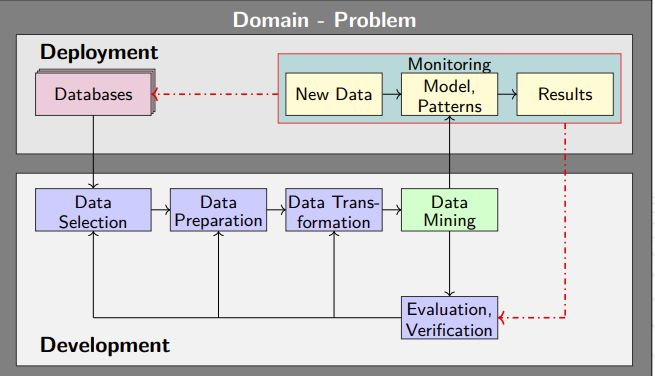
\includegraphics[width=\textwidth]{Images/KDD/KDDMonitoring}
	\caption{\textbf{Process Workflow}}
	
\end{figure}

\section{Introduction to \ac{kdd}}

Knowledge Discovery in Databases (\ac{kdd}) is a fundamental step in the broader knowledge discovery process. It refers to the systematic extraction of meaningful patterns, trends, and insights from large datasets. At its core, \ac{kdd} enables organizations and researchers to transform raw data into actionable knowledge. A key aspect of this process is data mining, which involves identifying interesting patterns within vast amounts of data.

By analyzing existing datasets, data mining facilitates the discovery of solutions to complex problems. This process involves leveraging historical data to build predictive models that anticipate future trends and behaviors. The ultimate objective of data mining is to uncover patterns that are not only valid and novel but also potentially useful and easily understandable. These insights often form the foundation for strategic decision-making across various industries.

\section{Types of Data Mining Tasks}

Data mining tasks can generally be classified into two primary categories: \textbf{descriptive tasks} and \textbf{predictive tasks}.

\subsection{Descriptive Tasks}
Descriptive data mining focuses on analyzing datasets to uncover inherent patterns and summarize their properties. These tasks help characterize the general attributes of data, providing insights into the underlying structure of the database. For example, clustering techniques can group similar data points, offering a better understanding of the dataset's composition.

\subsection{Predictive Tasks}
Predictive data mining, on the other hand, involves using historical data to forecast unknown or future trends. These tasks rely on identifying relationships between variables to make informed predictions. For instance, regression and classification models can predict customer behavior, sales trends, or market dynamics \cite{Fezari:2018}.

\section{Applications of Data Mining}

Data mining finds extensive applications across numerous industries, including:

\begin{itemize}
	\item \textbf{Healthcare:}  
	In medicine, data mining assists in analyzing patient records to predict disease progression, improve diagnostics, and tailor treatment plans. By identifying patterns in medical histories, healthcare providers can enhance patient care and operational efficiency.
	
	\item \textbf{Retail and Marketing:}  
	Retailers use data mining to understand consumer behavior, optimize pricing strategies, and personalize marketing campaigns. Analyzing sales data helps identify purchasing patterns, leading to better inventory management and targeted promotions.
	
	\item \textbf{Finance:}  
	In the financial sector, data mining plays a crucial role in fraud detection, credit scoring, and risk assessment. By analyzing transaction patterns, banks and financial institutions can mitigate risks and improve decision-making.
	
	\item \textbf{Telecommunications:}  
	Telecommunications companies use data mining to analyze customer usage patterns, predict churn rates, and improve service quality. These insights enable companies to develop more effective customer retention strategies.
	
	\item \textbf{Scientific Research:}  
	In science, data mining facilitates the analysis of large-scale datasets to uncover patterns and correlations that drive discoveries and innovations.
\end{itemize}

The insights derived from data mining empower organizations to improve profitability, enhance customer satisfaction, and optimize operations. The following sections delve deeper into specific data mining tasks and their methodologies.
	
\section{KDD for Magic Wand Project}
	
	The integration of Knowledge Discovery in Databases (\ac{kdd}) is a cornerstone in optimizing the design and performance of our Magic Wand project. This project leverages the Arduino Nano BLE 33, equipped with an accelerometer, to enable on-device gesture recognition. Through the application of \ac{kdd}, meaningful insights are derived from the extensive dataset generated by the device's accelerometer, enabling the seamless recognition and classification of predefined gestures.
	
	\subsection{Understanding Descriptive and Predictive Tasks}
	
	The application of \ac{kdd} in the Magic Wand project involves two primary categories of data mining tasks: descriptive and predictive.
	
	\begin{itemize}
		\item \textbf{Descriptive Tasks:}  
		Descriptive tasks focus on analyzing accelerometer data to uncover inherent functional patterns. These patterns help characterize the general properties of hand movements, offering valuable insights into the gestures' nature and variations. For instance, clustering similar motion patterns can highlight commonalities in user behavior, aiding in feature engineering for the recognition model.
		
		\item \textbf{Predictive Tasks:}  
		Predictive tasks utilize historical accelerometer data to anticipate future trends and behaviors. In the Magic Wand project, predictive modeling enables the system to identify and classify gestures in real time. By training the model on labeled datasets, it becomes capable of recognizing both simple and complex gestures with high accuracy.
	\end{itemize}
	
	\subsection{Applications of Data Mining in Gesture Recognition}
	
	Data mining, as a key component of \ac{kdd}, empowers the Magic Wand project to extract meaningful patterns from raw accelerometer data. This capability is instrumental in recognizing valid and novel hand gestures. The process involves feature extraction, pattern identification, and classification to ensure precise gesture recognition. By enhancing the accuracy and responsiveness of the system, data mining significantly improves user experience and system reliability \cite{Fezari:2018}.
	
	\subsection{Real-world Impact in Various Domains}
	
	The insights derived through \ac{kdd} extend the Magic Wand project's potential applications across multiple industries:
	
	\begin{itemize}
		\item \textbf{Healthcare:}  
		Gesture recognition systems powered by \ac{kdd} can assist in physical therapy, enabling patients to perform prescribed exercises while the system monitors and evaluates their movements.
		
		\item \textbf{Retail and Marketing:}  
		Retail environments can benefit from gesture-based interaction systems, such as virtual assistants or kiosks that respond to user gestures for navigation or selection.
		
		\item \textbf{Finance:}  
		In banking and finance, gesture recognition can facilitate secure authentication mechanisms and improve accessibility for individuals with disabilities.
		
		\item \textbf{Telecommunications:}  
		Gesture-based controls powered by data mining can enhance user interaction with smart devices, improving accessibility and functionality.
		
		\item \textbf{Science and Education:}  
		Gesture recognition systems can be used in educational tools to provide interactive learning experiences, especially in virtual or augmented reality environments \cite{Fezari:2018}.
	\end{itemize}
	\subsection{CRISP-DM}
The CRISP-DM process was developed by the means of the effort of a consortium initially composed with DaimlerChrysler, SPSS, and NCR. CRISP-DM stands for \textbf{Cross-Industry Standard Process for Data Mining}. It consists of a cycle that comprises six stages (Figure~2):  

\begin{enumerate}
    \item \textbf{Business understanding} – This initial phase focuses on understanding the project objectives and requirements from a business perspective, then converting this knowledge into a data mining problem definition and a preliminary plan designed to achieve the objectives.  

    \item \textbf{Data understanding} – The data understanding phase starts with an initial data collection and proceeds with activities in order to get familiar with the data, to identify data quality problems, to discover first insights into the data, or to detect interesting subsets to form hypotheses for hidden information.  

    \item \textbf{Data preparation} – The data preparation phase covers all activities to construct the final dataset from the initial raw data.  

    \item \textbf{Modeling} – In this phase, various modeling techniques are selected and applied, and their parameters are calibrated to optimal values.  

    \item \textbf{Evaluation} – At this stage, the model (or models) obtained is more thoroughly evaluated, and the steps executed to construct the model are reviewed to be certain it properly achieves the business objectives.  

    \item \textbf{Deployment} – Creation of the model is generally not the end of the project. Even if the purpose of the model is to increase knowledge of the data, the knowledge gained will need to be organized and presented in a way that the customer can use it.  
\end{enumerate}

 

\begin{figure}[h]
    \centering
    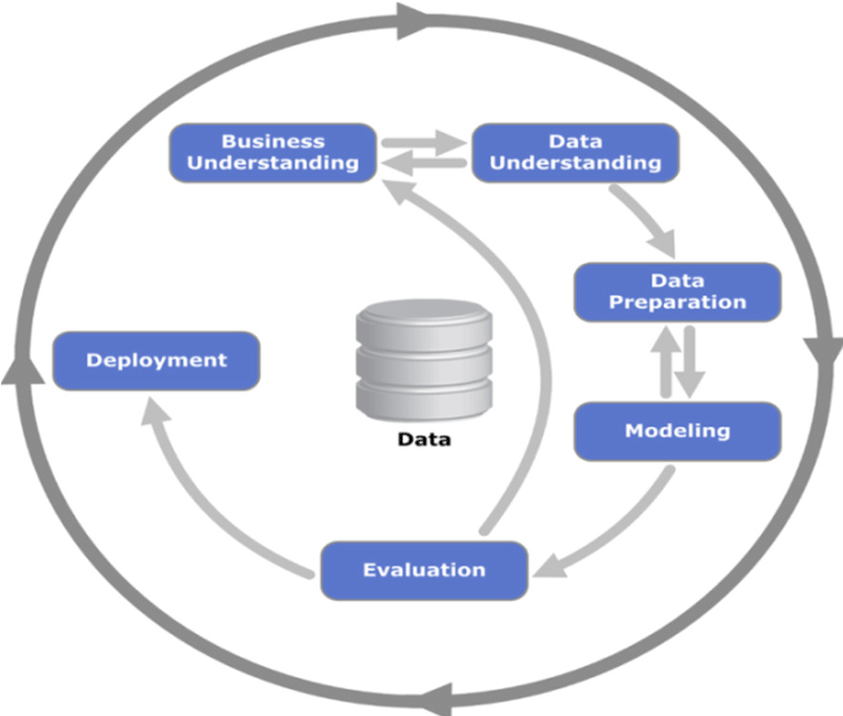
\includegraphics[width=0.8\textwidth]{Images/Methodology/figure2.png}
    \caption{The CRISP-DM life cycle (Chapman et al., 2000)}
\end{figure}

The sequence of the six stages is not rigid, as is schematized in Figure~2. CRISP-DM is extremely complete and documented. All its stages are duly organized, structured, and defined, allowing that a project could be easily understood or revised (Santos \& Azevedo, 2005). Although the CRISP-DM process is independent from the DM chosen tool, it is linked to the SPSS Clementine software.  


\subsection{Comparison of KDD and CRISP-DM}
\begin{table}[h!]
    \centering
    \begin{tabular}{@{}p{3.5cm}p{5.5cm}p{5.5cm}@{}}
        \toprule
        \textbf{Aspect} & \textbf{KDD (Knowledge Discovery in Databases)} & \textbf{CRISP-DM (Cross-Industry Standard Process for Data Mining)} \\ \midrule
        \textbf{Origin and Scope} & Focused on the overall process of extracting knowledge from databases. & Aimed at structuring data mining projects in a business or industrial setting. \\ \midrule
        \textbf{Phases} & 
        \begin{enumerate}
            \item Data Selection
            \item Data Preprocessing
            \item Data Transformation
            \item Data Mining
            \item Interpretation/Evaluation
        \end{enumerate} &
        \begin{enumerate}
            \item Business Understanding
            \item Data Understanding
            \item Data Preparation
            \item Modeling
            \item Evaluation
            \item Deployment
        \end{enumerate} \\ \midrule
        \textbf{Flexibility} & High flexibility, emphasizes iterative exploration and hypothesis testing. & Prescriptive and structured, with an emphasis on well-documented steps for business clarity. \\ \midrule
        \textbf{Tool Independence} & Independent of tools and platforms. & Initially linked to SPSS Clementine (now IBM SPSS Modeler). \\ \midrule
        \textbf{Target Audience} & Academics and technical experts focused on novel insights and experimental exploration. & Business professionals requiring a structured, repeatable process for solving problems. \\ \midrule
        \textbf{Documentation Emphasis} & Less formalized; focuses on the iterative discovery of knowledge. & High emphasis on documentation for ease of project understanding and reproducibility. \\ 
        \bottomrule
    \end{tabular}
    \caption{Comparison of KDD and CRISP-DM}
    \label{tab:comparison}
\end{table}

\subsection{Why KDD is Better for the Magic Wand Project}
The magic wand project using the Arduino Nano 33 BLE Sense involves real-time sensor data processing and gesture recognition. Below are key reasons why KDD is better suited:

\begin{enumerate}
    \item \textbf{Focus on Sensor Data Processing} 
    The Arduino Nano 33 BLE Sense provides raw sensor data (e.g., accelerometer, gyroscope, magnetometer). KDD emphasizes \textit{data preprocessing} and \textit{transformation}, which are essential for converting raw data into meaningful features (e.g., gesture patterns). KDD's iterative nature allows for fine-tuning these transformations, crucial for a real-time system like the magic wand.

    \item \textbf{Exploratory Nature of KDD} 
    The magic wand project involves \textit{exploring gestures} and creating patterns using embedded sensors. KDD allows repeated hypothesis testing and refinement, enabling the discovery of novel gesture mappings or better feature extraction techniques.

    \item \textbf{Less Emphasis on Business Objectives} 
    CRISP-DM’s \textit{business understanding phase} is less relevant for this project, which is \textit{experimental and technical} rather than business-driven. KDD focuses directly on the data and knowledge discovery, aligning well with the goals of the magic wand.

    \item \textbf{Tool Independence} 
    KDD is tool-agnostic and compatible with \textit{open-source platforms} like Arduino. CRISP-DM, initially linked to SPSS Clementine (a proprietary tool), is less adaptable for hardware-based projects.

    \item \textbf{Iterative Feedback} 
    In KDD, the iterative cycle between preprocessing, transformation, and data mining is critical for adapting to sensor noise or calibration changes. This feedback loop is vital for optimizing gesture recognition in the magic wand project.
\end{enumerate}

KDD is better suited for the \textit{magic wand project using Arduino Nano 33 BLE Sense} because it provides the flexibility needed to work with raw sensor data, emphasizes preprocessing and transformation, and facilitates iterative exploration and optimization of gesture recognition models. These aspects align closely with the challenges and goals of the project, making KDD the ideal methodology.


\subsection{ML Pipeline}

\subsection{1. Data Selection}
\textbf{Objective}: Identify and collect relevant sensor data.  
\begin{itemize}
    \item Use the embedded sensors (e.g., accelerometer, gyroscope, magnetometer) on the Arduino Nano 33 BLE Sense.
    \item Define the gestures to be recognized (e.g., wave, circle, swipe).
    \item Collect sensor data for each gesture, ensuring variation in speed, orientation, and user input.
    \item Store raw data for each axis (X, Y, Z) over time.
\end{itemize}
\textbf{Tools}: Arduino IDE for data logging, serial communication, or an SD card for storage.

\subsection{2. Data Preprocessing}
\textbf{Objective}: Clean and prepare raw sensor data for analysis.  
\begin{itemize}
    \item \textbf{Data Cleaning}: Remove noise and outliers using filters (e.g., low-pass filter to remove high-frequency noise).
    \item \textbf{Data Resampling}: Normalize sampling rates for consistent data across all gestures.
    \item \textbf{Windowing}: Segment data into fixed-size time windows (e.g., 1-second windows) to capture meaningful patterns.
    \item \textbf{Scaling}: Normalize sensor values to a consistent range (e.g., [-1, 1] or [0, 1]).
\end{itemize}
\textbf{Tools}: Python (e.g., NumPy, Pandas), Arduino libraries (e.g., filters).

\subsection{3. Data Transformation}
\textbf{Objective}: Extract features from the preprocessed data.  
\begin{itemize}
    \item Compute statistical features like mean, variance, standard deviation, energy, and entropy for each window.
    \item Calculate domain-specific features (e.g., Fast Fourier Transform (FFT) for frequency analysis).
    \item Combine features from multiple sensors (e.g., accelerometer + gyroscope).
    \item Encode gestures into labeled data (e.g., ``gesture\_1'', ``gesture\_2'').
\end{itemize}
\textbf{Tools}: Python (e.g., SciPy, sklearn), MATLAB (if needed).

\subsection{4. Data Mining (Modeling)}
\textbf{Objective}: Train a machine learning model to classify gestures.  
\begin{itemize}
    \item \textbf{Split the dataset}: Use an 80-20 train-test split.
    \item \textbf{Model Selection}: Choose lightweight models suitable for edge devices, such as:
          \begin{itemize}
              \item Decision Trees
              \item Random Forest
              \item k-Nearest Neighbors (k-NN)
              \item Neural Networks (e.g., TensorFlow Lite for microcontrollers)
          \end{itemize}
    \item \textbf{Training}: Optimize hyperparameters (e.g., tree depth, number of neighbors).
    \item \textbf{Validation}: Use cross-validation to ensure model generalization.
\end{itemize}
\textbf{Tools}: TensorFlow Lite, Edge Impulse, or sklearn.

\subsection{5. Interpretation/Evaluation}
\textbf{Objective}: Evaluate model performance and refine it.  
\begin{itemize}
    \item \textbf{Metrics}:
          \begin{itemize}
              \item Accuracy, precision, recall, and F1-score.
              \item Confusion matrix to analyze gesture misclassifications.
              \item Latency and memory usage to ensure real-time performance on the Arduino.
          \end{itemize}
    \item \textbf{Steps}:
          \begin{itemize}
              \item Test the model on unseen gesture data.
              \item Evaluate performance under real-world conditions (e.g., different lighting or motion speeds).
          \end{itemize}
\end{itemize}
\textbf{Tools}: Arduino Nano's onboard resources for testing, Python for analysis.

\subsection{6. Deployment}
\textbf{Objective}: Deploy the trained model onto the Arduino Nano 33 BLE Sense.  
\begin{itemize}
    \item Convert the model into a format suitable for the Arduino (e.g., TensorFlow Lite format).
    \item Integrate the model with gesture recognition logic using Arduino libraries.
    \item Test gesture recognition in real-time and refine thresholds or logic as needed.
    \item Optimize for power consumption and memory.
\end{itemize}
\textbf{Tools}: TensorFlow Lite for Microcontrollers, Arduino IDE, Edge Impulse Studio.

\subsection{Pipeline Flow Diagram}
\[
\text{Sensor Data Collection} \rightarrow \text{Preprocessing} \rightarrow \text{Feature Extraction} \rightarrow \text{Model Training} \rightarrow \text{Evaluation} \rightarrow \text{Deployment}
\]

	
	\subsection{Conclusion}
	
	By employing the principles of \ac{kdd}, the Magic Wand project effectively harnesses the potential of data mining to analyze and understand hand movements. This approach ensures accurate and real-time gesture recognition, paving the way for innovative applications across diverse industries.
	

